% GNUPLOT: LaTeX picture with Postscript
\begingroup
  \makeatletter
  \providecommand\color[2][]{%
    \GenericError{(gnuplot) \space\space\space\@spaces}{%
      Package color not loaded in conjunction with
      terminal option `colourtext'%
    }{See the gnuplot documentation for explanation.%
    }{Either use 'blacktext' in gnuplot or load the package
      color.sty in LaTeX.}%
    \renewcommand\color[2][]{}%
  }%
  \providecommand\includegraphics[2][]{%
    \GenericError{(gnuplot) \space\space\space\@spaces}{%
      Package graphicx or graphics not loaded%
    }{See the gnuplot documentation for explanation.%
    }{The gnuplot epslatex terminal needs graphicx.sty or graphics.sty.}%
    \renewcommand\includegraphics[2][]{}%
  }%
  \providecommand\rotatebox[2]{#2}%
  \@ifundefined{ifGPcolor}{%
    \newif\ifGPcolor
    \GPcolortrue
  }{}%
  \@ifundefined{ifGPblacktext}{%
    \newif\ifGPblacktext
    \GPblacktexttrue
  }{}%
  % define a \g@addto@macro without @ in the name:
  \let\gplgaddtomacro\g@addto@macro
  % define empty templates for all commands taking text:
  \gdef\gplbacktext{}%
  \gdef\gplfronttext{}%
  \makeatother
  \ifGPblacktext
    % no textcolor at all
    \def\colorrgb#1{}%
    \def\colorgray#1{}%
  \else
    % gray or color?
    \ifGPcolor
      \def\colorrgb#1{\color[rgb]{#1}}%
      \def\colorgray#1{\color[gray]{#1}}%
      \expandafter\def\csname LTw\endcsname{\color{white}}%
      \expandafter\def\csname LTb\endcsname{\color{black}}%
      \expandafter\def\csname LTa\endcsname{\color{black}}%
      \expandafter\def\csname LT0\endcsname{\color[rgb]{1,0,0}}%
      \expandafter\def\csname LT1\endcsname{\color[rgb]{0,1,0}}%
      \expandafter\def\csname LT2\endcsname{\color[rgb]{0,0,1}}%
      \expandafter\def\csname LT3\endcsname{\color[rgb]{1,0,1}}%
      \expandafter\def\csname LT4\endcsname{\color[rgb]{0,1,1}}%
      \expandafter\def\csname LT5\endcsname{\color[rgb]{1,1,0}}%
      \expandafter\def\csname LT6\endcsname{\color[rgb]{0,0,0}}%
      \expandafter\def\csname LT7\endcsname{\color[rgb]{1,0.3,0}}%
      \expandafter\def\csname LT8\endcsname{\color[rgb]{0.5,0.5,0.5}}%
    \else
      % gray
      \def\colorrgb#1{\color{black}}%
      \def\colorgray#1{\color[gray]{#1}}%
      \expandafter\def\csname LTw\endcsname{\color{white}}%
      \expandafter\def\csname LTb\endcsname{\color{black}}%
      \expandafter\def\csname LTa\endcsname{\color{black}}%
      \expandafter\def\csname LT0\endcsname{\color{black}}%
      \expandafter\def\csname LT1\endcsname{\color{black}}%
      \expandafter\def\csname LT2\endcsname{\color{black}}%
      \expandafter\def\csname LT3\endcsname{\color{black}}%
      \expandafter\def\csname LT4\endcsname{\color{black}}%
      \expandafter\def\csname LT5\endcsname{\color{black}}%
      \expandafter\def\csname LT6\endcsname{\color{black}}%
      \expandafter\def\csname LT7\endcsname{\color{black}}%
      \expandafter\def\csname LT8\endcsname{\color{black}}%
    \fi
  \fi
  \setlength{\unitlength}{0.0500bp}%
  \begin{picture}(7370.00,9636.00)%
    \gplgaddtomacro\gplbacktext{%
      \csname LTb\endcsname%
      \put(-120,7050){\makebox(0,0)[r]{\strut{}-60}}%
      \csname LTb\endcsname%
      \put(-120,7620){\makebox(0,0)[r]{\strut{}-40}}%
      \csname LTb\endcsname%
      \put(-120,8190){\makebox(0,0)[r]{\strut{}-20}}%
      \csname LTb\endcsname%
      \put(-120,8760){\makebox(0,0)[r]{\strut{} 0}}%
      \csname LTb\endcsname%
      \put(-120,9330){\makebox(0,0)[r]{\strut{} 20}}%
      \put(0,6565){\makebox(0,0){\strut{}}}%
      \put(245,6565){\makebox(0,0){\strut{}}}%
      \put(491,6565){\makebox(0,0){\strut{}}}%
      \put(736,6565){\makebox(0,0){\strut{}}}%
      \put(981,6565){\makebox(0,0){\strut{}}}%
      \put(1227,6565){\makebox(0,0){\strut{}}}%
      \put(1472,6565){\makebox(0,0){\strut{}}}%
      \put(1717,6565){\makebox(0,0){\strut{}}}%
      \put(1962,6565){\makebox(0,0){\strut{}}}%
      \put(2208,6565){\makebox(0,0){\strut{}}}%
      \put(2453,6565){\makebox(0,0){\strut{}}}%
      \put(245,9815){\makebox(0,0){\strut{} 0}}%
      \put(736,9815){\makebox(0,0){\strut{} 2}}%
      \put(1227,9815){\makebox(0,0){\strut{} 4}}%
      \put(1717,9815){\makebox(0,0){\strut{} 6}}%
      \put(2208,9815){\makebox(0,0){\strut{} 8}}%
      \put(-700,8190){\rotatebox{-270}{\makebox(0,0){\strut{}Abweichung [MHz]}}}%
      \put(245,7193){\makebox(0,0)[l]{\strut{}\tiny{max. m"ogl. Abweichung: $11.2$ MHz}}}%
    }%
    \gplgaddtomacro\gplfronttext{%
      \csname LTb\endcsname%
      \put(1670,7805){\makebox(0,0)[r]{\strut{}\tiny{zw. Fringes [MHz]}}}%
      \csname LTb\endcsname%
      \put(1670,7605){\makebox(0,0)[r]{\strut{}\tiny{absolut [MHz]}}}%
    }%
    \gplgaddtomacro\gplbacktext{%
      \csname LTb\endcsname%
      \put(2334,7050){\makebox(0,0)[r]{\strut{}}}%
      \csname LTb\endcsname%
      \put(2334,7620){\makebox(0,0)[r]{\strut{}}}%
      \csname LTb\endcsname%
      \put(2334,8190){\makebox(0,0)[r]{\strut{}}}%
      \csname LTb\endcsname%
      \put(2334,8760){\makebox(0,0)[r]{\strut{}}}%
      \csname LTb\endcsname%
      \put(2334,9330){\makebox(0,0)[r]{\strut{}}}%
      \put(2454,6565){\makebox(0,0){\strut{}}}%
      \put(2699,6565){\makebox(0,0){\strut{}}}%
      \put(2945,6565){\makebox(0,0){\strut{}}}%
      \put(3190,6565){\makebox(0,0){\strut{}}}%
      \put(3435,6565){\makebox(0,0){\strut{}}}%
      \put(3681,6565){\makebox(0,0){\strut{}}}%
      \put(3926,6565){\makebox(0,0){\strut{}}}%
      \put(4171,6565){\makebox(0,0){\strut{}}}%
      \put(4416,6565){\makebox(0,0){\strut{}}}%
      \put(4662,6565){\makebox(0,0){\strut{}}}%
      \put(4907,6565){\makebox(0,0){\strut{}}}%
      \put(2699,9815){\makebox(0,0){\strut{} 0}}%
      \put(3190,9815){\makebox(0,0){\strut{} 2}}%
      \put(3681,9815){\makebox(0,0){\strut{} 4}}%
      \put(4171,9815){\makebox(0,0){\strut{} 6}}%
      \put(4662,9815){\makebox(0,0){\strut{} 8}}%
      \put(3680,10214){\makebox(0,0){\strut{}Scan Position [GHz]}}%
      \put(2699,7193){\makebox(0,0)[l]{\strut{}\tiny{max. m"ogl. Abweichung: $54.2$ MHz}}}%
    }%
    \gplgaddtomacro\gplfronttext{%
    }%
    \gplgaddtomacro\gplbacktext{%
      \csname LTb\endcsname%
      \put(4788,7050){\makebox(0,0)[r]{\strut{}}}%
      \csname LTb\endcsname%
      \put(4788,7620){\makebox(0,0)[r]{\strut{}}}%
      \csname LTb\endcsname%
      \put(4788,8190){\makebox(0,0)[r]{\strut{}}}%
      \csname LTb\endcsname%
      \put(4788,8760){\makebox(0,0)[r]{\strut{}}}%
      \csname LTb\endcsname%
      \put(4788,9330){\makebox(0,0)[r]{\strut{}}}%
      \put(4908,6565){\makebox(0,0){\strut{}}}%
      \put(5152,6565){\makebox(0,0){\strut{}}}%
      \put(5396,6565){\makebox(0,0){\strut{}}}%
      \put(5640,6565){\makebox(0,0){\strut{}}}%
      \put(5884,6565){\makebox(0,0){\strut{}}}%
      \put(6128,6565){\makebox(0,0){\strut{}}}%
      \put(6373,6565){\makebox(0,0){\strut{}}}%
      \put(6617,6565){\makebox(0,0){\strut{}}}%
      \put(6861,6565){\makebox(0,0){\strut{}}}%
      \put(7105,6565){\makebox(0,0){\strut{}}}%
      \put(7349,6565){\makebox(0,0){\strut{}}}%
      \put(5152,9815){\makebox(0,0){\strut{} 0}}%
      \put(5640,9815){\makebox(0,0){\strut{} 2}}%
      \put(6128,9815){\makebox(0,0){\strut{} 4}}%
      \put(6617,9815){\makebox(0,0){\strut{} 6}}%
      \put(7105,9815){\makebox(0,0){\strut{} 8}}%
      \put(5152,7193){\makebox(0,0)[l]{\strut{}\tiny{max. m"ogl. Abweichung: $79.8$ MHz}}}%
    }%
    \gplgaddtomacro\gplfronttext{%
    }%
    \gplgaddtomacro\gplbacktext{%
      \csname LTb\endcsname%
      \put(-120,3291){\makebox(0,0)[r]{\strut{}10}}%
      \csname LTb\endcsname%
      \put(-120,3673){\makebox(0,0)[r]{\strut{}20}}%
      \csname LTb\endcsname%
      \put(-120,4054){\makebox(0,0)[r]{\strut{}30}}%
      \csname LTb\endcsname%
      \put(-120,4436){\makebox(0,0)[r]{\strut{}40}}%
      \csname LTb\endcsname%
      \put(-120,4817){\makebox(0,0)[r]{\strut{}50}}%
      \csname LTb\endcsname%
      \put(-120,5199){\makebox(0,0)[r]{\strut{}60}}%
      \csname LTb\endcsname%
      \put(-120,5580){\makebox(0,0)[r]{\strut{}70}}%
      \csname LTb\endcsname%
      \put(-120,5962){\makebox(0,0)[r]{\strut{}80}}%
      \csname LTb\endcsname%
      \put(-120,6343){\makebox(0,0)[r]{\strut{}90}}%
      \put(0,2710){\makebox(0,0){\strut{}}}%
      \put(736,2710){\makebox(0,0){\strut{}}}%
      \put(1471,2710){\makebox(0,0){\strut{}}}%
      \put(2207,2710){\makebox(0,0){\strut{}}}%
      \put(2942,2710){\makebox(0,0){\strut{}}}%
      \put(3678,2710){\makebox(0,0){\strut{}}}%
      \put(4414,2710){\makebox(0,0){\strut{}}}%
      \put(5149,2710){\makebox(0,0){\strut{}}}%
      \put(5885,2710){\makebox(0,0){\strut{}}}%
      \put(6620,2710){\makebox(0,0){\strut{}}}%
      \put(7356,2710){\makebox(0,0){\strut{}}}%
      \put(736,6725){\makebox(0,0){\strut{}}}%
      \put(2207,6725){\makebox(0,0){\strut{}}}%
      \put(3678,6725){\makebox(0,0){\strut{}}}%
      \put(5149,6725){\makebox(0,0){\strut{}}}%
      \put(6620,6725){\makebox(0,0){\strut{}}}%
      \put(-580,4817){\rotatebox{-270}{\makebox(0,0){\strut{}max. Scanfehler [MHz]}}}%
    }%
    \gplgaddtomacro\gplfronttext{%
    }%
    \gplgaddtomacro\gplbacktext{%
      \csname LTb\endcsname%
      \put(-120,1234){\makebox(0,0)[r]{\strut{}-6}}%
      \csname LTb\endcsname%
      \put(-120,1468){\makebox(0,0)[r]{\strut{}-4}}%
      \csname LTb\endcsname%
      \put(-120,1702){\makebox(0,0)[r]{\strut{}-2}}%
      \csname LTb\endcsname%
      \put(-120,1936){\makebox(0,0)[r]{\strut{}0}}%
      \csname LTb\endcsname%
      \put(-120,2169){\makebox(0,0)[r]{\strut{}2}}%
      \csname LTb\endcsname%
      \put(-120,2403){\makebox(0,0)[r]{\strut{}4}}%
      \csname LTb\endcsname%
      \put(-120,2637){\makebox(0,0)[r]{\strut{}6}}%
      \put(0,800){\makebox(0,0){\strut{}17:00}}%
      \put(736,800){\makebox(0,0){\strut{}17:30}}%
      \put(1471,800){\makebox(0,0){\strut{}18:00}}%
      \put(2207,800){\makebox(0,0){\strut{}18:30}}%
      \put(2942,800){\makebox(0,0){\strut{}19:00}}%
      \put(3678,800){\makebox(0,0){\strut{}19:30}}%
      \put(4414,800){\makebox(0,0){\strut{}20:00}}%
      \put(5149,800){\makebox(0,0){\strut{}20:30}}%
      \put(5885,800){\makebox(0,0){\strut{}21:00}}%
      \put(6620,800){\makebox(0,0){\strut{}21:30}}%
      \put(7356,800){\makebox(0,0){\strut{}22:00}}%
      \put(736,2871){\makebox(0,0){\strut{}}}%
      \put(2207,2871){\makebox(0,0){\strut{}}}%
      \put(3678,2871){\makebox(0,0){\strut{}}}%
      \put(5149,2871){\makebox(0,0){\strut{}}}%
      \put(6620,2871){\makebox(0,0){\strut{}}}%
      \put(-580,1935){\rotatebox{-270}{\makebox(0,0){\strut{}FSR-Fehler [MHz]}}}%
      \put(3678,500){\makebox(0,0){\strut{}Zeit}}%
    }%
    \gplgaddtomacro\gplfronttext{%
    }%
    \gplbacktext
    \put(0,0){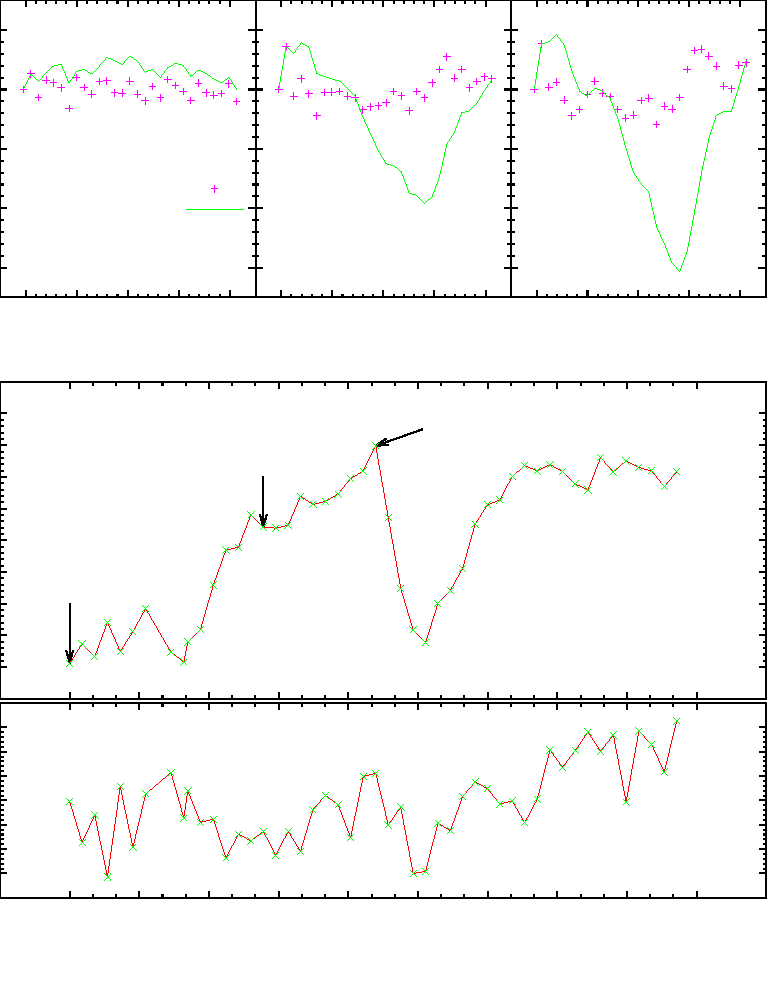
\includegraphics{linearitaet_verlauf}}%
    \gplfronttext
  \end{picture}%
\endgroup
